\documentclass[11pt, a4paper]{article}

\usepackage{graphicx}
\usepackage[a4paper,top=3cm,bottom=2cm,left=2cm,right=2cm,marginparwidth=1.75cm]{geometry}
\usepackage[english]{babel}
\usepackage[utf8x]{inputenc}
\usepackage{subfig}
\usepackage{float}
\usepackage{amsmath}
\usepackage{amssymb}
\usepackage{mhchem}
\usepackage{hyperref}
\usepackage{tikz}
\usepackage{cancel}
\usepackage{bm}

\graphicspath{ {./images} }
\newcommand*{\qed}{\hfill\ensuremath{\quad\square}}%
\newcommand*{\rad}{\ensuremath{\,\text{rad}}}
\newcommand*{\R}{\ensuremath{\mathbb{R}}}
\newcommand*{\C}{\ensuremath{\mathbb{C}}}
\renewcommand*{\Re}{\operatorname{Re}}
\renewcommand*{\Im}{\operatorname{Im}}
\renewcommand*{\epsilon}{\varepsilon}
\renewcommand*{\phi}{\varphi}
\renewcommand*{\d}{\text{d}}

\DeclareRobustCommand{\uvec}[1]{{%
  \ifcat\relax\noexpand#1%
    % it should be a Greek letter
    \bm{\hat{#1}}%
  \else
    \ifcsname uvec#1\endcsname
      \csname uvec#1\endcsname
    \else
      \bm{\hat{\mathbf{#1}}}%
     \fi
   \fi
}}

\makeatletter
\renewcommand*\env@matrix[1][*\c@MaxMatrixCols c]{%
  \hskip -\arraycolsep
  \let\@ifnextchar\new@ifnextchar
  \array{#1}}
\makeatother

\newtheorem{theorem}{Theorem}
\numberwithin{equation}{section}
\numberwithin{figure}{section}

%------------------------------------------------
%Templates for images and figures
% \begin{figure}[h]
%   \centering
%   \subfloat[caption 1]{{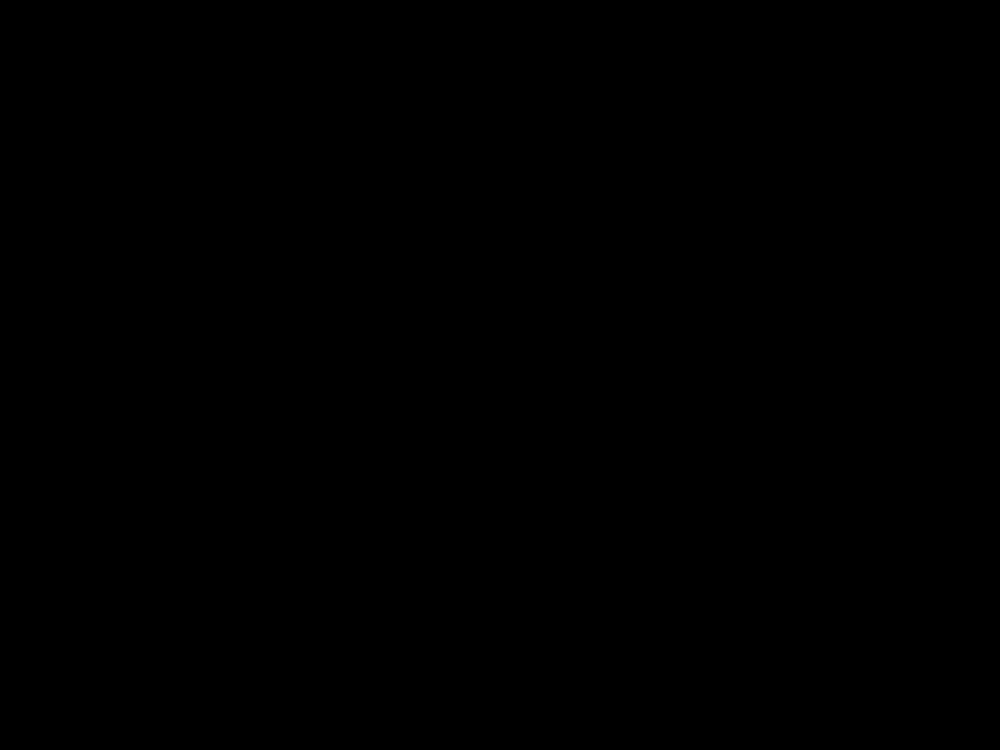
\includegraphics[width=30mm]{images/placeholder.png}}}%
%   \qquad
%   \subfloat[caption 2]{{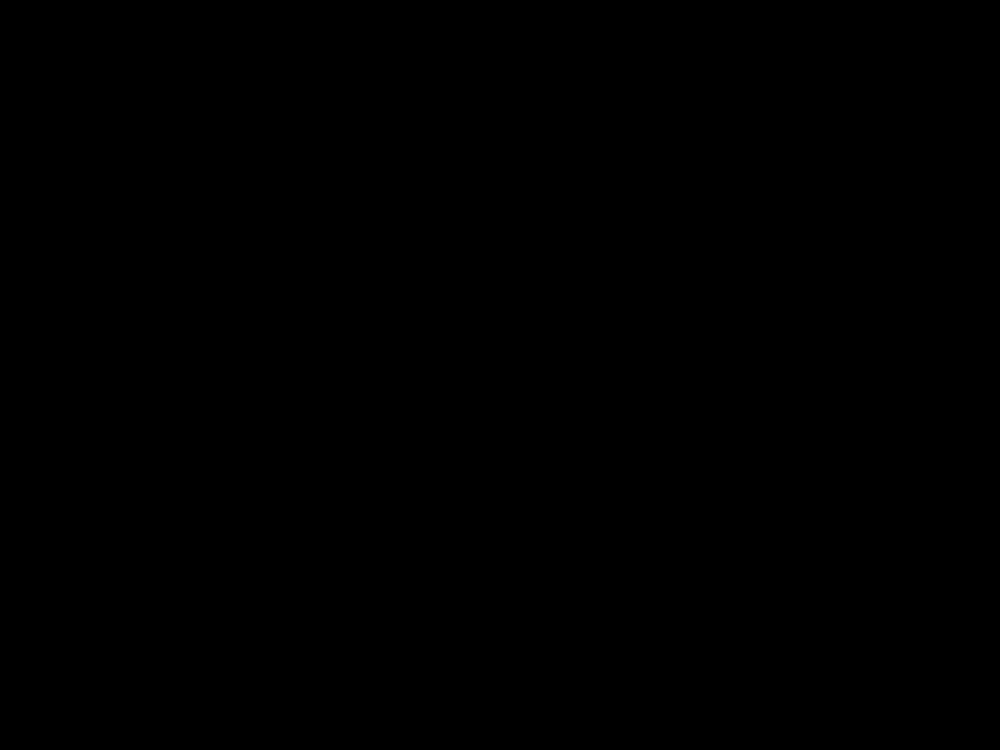
\includegraphics[width=30mm]{images/placeholder.png}}}%
%   \caption{Description}
% \end{figure}

% \begin{figure}[h]
%   \centerline{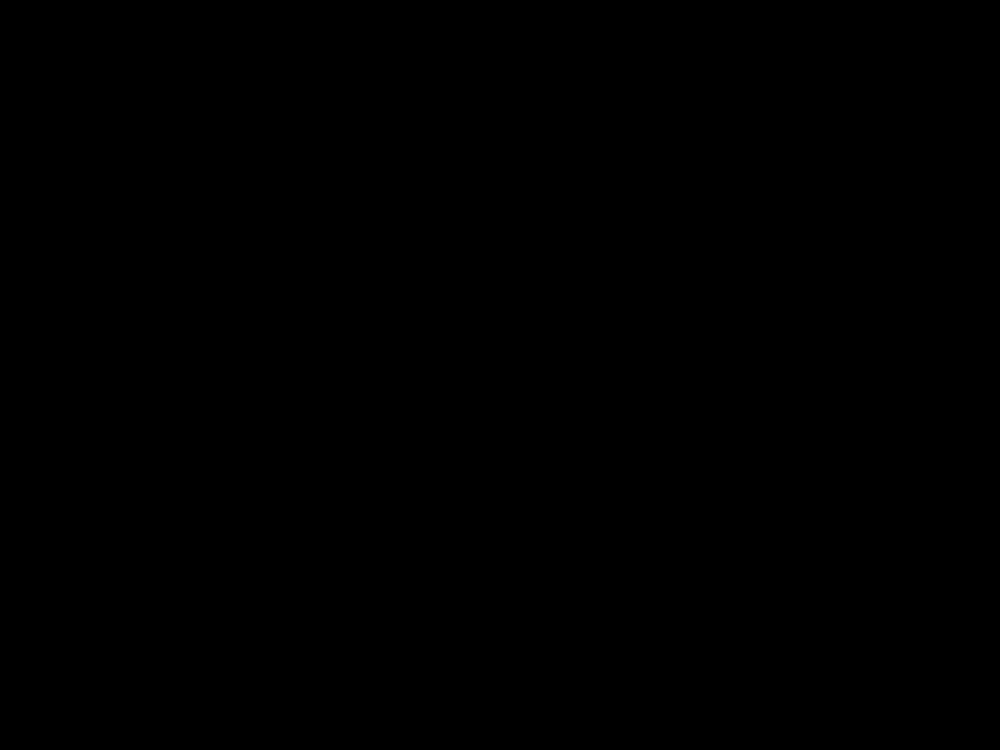
\includegraphics[width=50mm]{images/placeholder.png}}
%   \caption{Description}
% \end{figure}

%Template for a simple table 
%\begin{table}[h]
%   \caption{Description} %title of the table
%   \centering % centering table
%   \begin{tabular}{l rr} % creating three columns
%     \hline\hline %inserting double-line
%     & & \\ [0.5ex] % Insert half line vertical spacing
%     \hline % inserts single-line
%     & & \\ 
%     & & \\
%     & & \\
%     & & \\
%   \hline % inserts single-line
%   \end{tabular}
%   \label{tab:hresult}
% \end{table}
%-----------------------------------------------

\begin{document}

\setcounter{section}{2}

\section{Testing series for convergence}

\subsection{The integral test}
let $s_n$ be a series who is defined as follows:
\begin{equation}
  s_n = \sum_{n=1}^\infty \frac{1}{n^2} = 1 + \sum_{n=2}^\infty \frac{1}{n^2}
\end{equation}
Now let's compare this series to the graph of $f(x) = \frac{1}{x^2}$ on the interval $[1, \infty)$. This can be found in the figure below.
\begin{figure}[h]
  \centerline{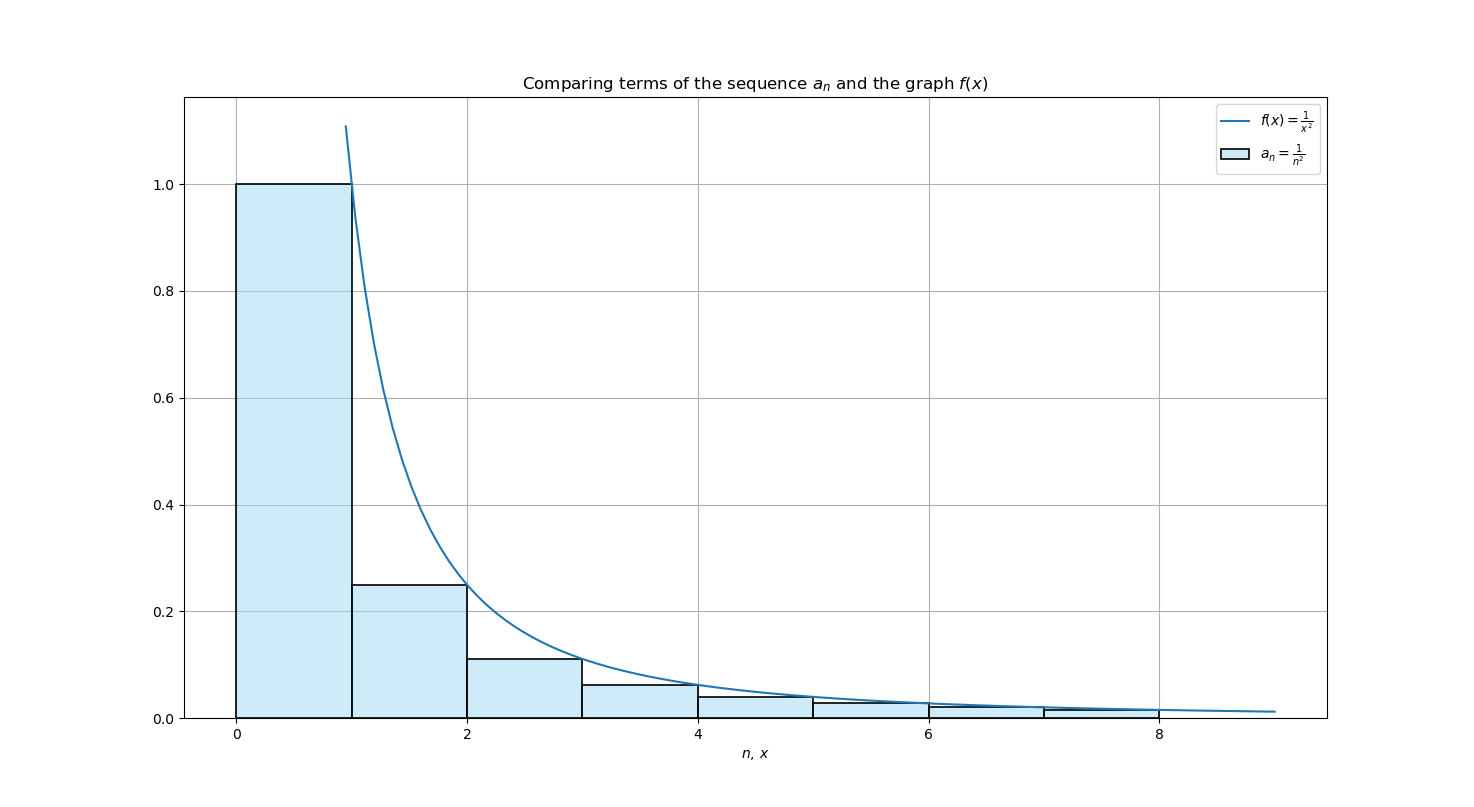
\includegraphics[width=120mm]{images/graph_1.png}}
  \caption{The graph $f(x)=\frac{1}{x^2}$ as compared to the series $ s_n = \sum_{n=1}^\infty \frac{1}{n^2}$}
\end{figure}
Using this figure we can easily see that the total area of the series must be less then the total area under the graph of $f(x)$. This means we end up with the following relation:
\begin{align}
  s_n &< \int_1^\infty f(x) \,\d x\\
  1 + \sum_{n=2}^\infty \frac{1}{n^2} &< 1 + \int_1^\infty \frac{1}{x^2} \,\d x\\ 
                                      &< 1 + 1 = 2 \notag
\end{align}
Thus the series $\sum_{n=1}^\infty \frac{1}{n^2}$ must converge since the integral of $f(x)$ also converges. We can state that it has a sum greater then 1 but smaller then 2. Computing the exact value of the series is outside of the scope of the course, however the answer is $\frac{\pi^2}{6}$. Look up the Basel problem if interested.\\
\begin{figure}[h]
  \centering
  \subfloat[$\sum_{n=1}^\infty f(n) \geq \int_1^\infty f(x) \,\d x$]{{\includegraphics[width=80mm]{images/Graph_2.png}}}%
  \qquad
  \subfloat[$\sum_{n=2}^\infty f(n) \leq \int_1^\infty f(x) \,\d x$]{{\includegraphics[width=80mm]{images/Graph_3.png}}}%
  \caption{The series $f(n)$ and the function $f(x)$ graphed twice for starting the series at $1$ and at $2$.}
\end{figure}
From these graphs we can easily find the following relation:
\begin{equation}
  \sum_{n=2}^\infty f(n) \leq \int_1^\infty f(x)\, \d x \leq \sum_{n=1}^\infty f(n)
\end{equation}
Let $f$ be a positive, continuous, (eventually) decreasing function on the interval $[1, \infty)$. Let $a_n = f(n)$. The series $\sum_{n=1}^\infty \ a_n$ converges iff the integral $\int_1^\infty f(x)\,\d x$ is convergent.\\
\\
\underline{Example:}
Find whether the following sum converges or diverges:
\begin{equation*}
  \sum_{n=1}^\infty \frac{1}{\sqrt{n+1}}
\end{equation*}
We compare this to the integral from 1 to infinity of the graph $f(x) = \frac{1}{\sqrt{x+1}}$. This gives:
\begin{align*}
  \int_1^\infty \frac{1}{\sqrt{x+1}}\,\d x &= \lim_{t\to\infty} \int_1^t \frac{1}{\sqrt{x+1}}\,\d x\\
                                           &= \lim_{t\to\infty} \left. 2\sqrt{x+1} \right|_1^t\\
                                           &= \infty
\end{align*}
Since $f(x)$, a continuous decreasing function on the interval $[1, \infty)$, diverges we can state that the sum $\sum_{n=1}^\infty \frac{1}{\sqrt{n+1}}$ must also diverge since it must be greater then the integral $\int_1^\infty f(x)\,\d x$.

\subsection{P-series and comparison to p-series}
Let's start with a question: for which value of $p$ is the series $\sum_{n=1}^\infty \frac{1}{n^p}$ convergent?\\
Right of the bat we notice 2 things:
\begin{itemize}
  \item $p=1$ gives us the harmonic series which we know diverges
  \item $p \leq 0$ has a general term that doesn't go to $0$ and thus can't converge
\end{itemize}
Let's apply the comparison to an integral to this series:
\begin{align}
  \int_1^\infty \frac{1}{x^p}\,\d x &= \lim_{t\to\infty}\int_1^t x^{-p}\,\d x \notag\\
                                    &= \lim_{t\to\infty} \left. \frac{x^{-p+1}}{-p+1} \right|_0^t
\end{align}
From this we can see that this limit converges if $p>1$. From this we can conclude that the series $\sum_{n=1}^\infty \frac{1}{n^p}$ is convergent iff\footnote{if and only if} $p>1$. This is a fact we can use in our analysis. Whenever we encounter a series which takes the form of the p-series we can conclude whether it converges or diverges based on the value of $p$ alone. Further analysis will then not be required.


\subsection{Estimating remainder of a series}
Let $a_k$ be some sequence. We can use this sequence to construct a series. Recall that the partial sum of a series is given as the first $n$ terms of the series. This leaves a remainder of the series from the term $n+1$ up untill $\infty$. We can express this as:
\begin{align}
  \sum_{k=1}^\infty a_k &= \sum_{k=1}^n a_k + \sum_{k=n+1}^\infty a_k \notag\\
                        &= s_n + R_n
\end{align}
Where $R_n$ is the remainder term of the series and $s_n$ the partial sum of the first $n$ terms. If $f$ is some continuous, positive, (eventually) decreasing function on the interval $[1, \infty)$ and $a_n = f(n)$:
\begin{equation}
  \int_{n+1}^\infty f(x)\,\d x \leq R_n \leq \int_{n}^\infty f(x)\,\d x
\end{equation}
We can add $s_n$ to all term of this expression and since $\sum_{k=1}^\infty a_k = s_n + R_n$ we can subsitute this back in to find:
\begin{equation}
  s_n + \int_{n+1}^\infty f(x)\,\d x \leq s \leq s_n +  \int_{n}^\infty f(x)\,\d x
\end{equation}

\underline{Example:} How many terms do we need to add up in te series $\sum_{n=1}^\infty \frac{1}{n^4}$ for $R_n < 10^{-3}$?
We start by applying the theorem we established earlier:
\begin{align*}
  \int_{n+1}^\infty \frac{1}{x^4}\,\d x \leq &R_n \leq \int_n^\infty \frac{1}{x^4}\,\d x\\
  \lim_{t \to\infty} \left. \frac{1}{3(x+1)^3} \right|_{n+1}^t \leq &R_n \leq \lim_{t\to\infty} \left. \frac{1}{3x^3} \right|_{n+1}^t\\
  \frac{1}{3(n+1)^3} \leq &R_n \leq \frac{1}{3n^3}
\end{align*}
We now found the expression for the upper and lower bound on the remainder term. From here we can try different values for $n$ either by hand or using a computer to find which value for $n$ statisfies the condition that $R_n < 10^{-3}$. We find that for $n=7$ we get:
\begin{align*}
  \frac{1}{3\cdot 8^3} \leq &R_7 \leq \frac{1}{3\cdot 7^3}
  0.00065 \leq R_7 \leq 0.00097 < 10^{-3}
\end{align*}
Thus by adding up the first $7$ terms of the series we get an answer which is within $10^{-3}$ of the exact answer. We can use this to find that:
\begin{equation*}
  \sum_{k=1}^7 \frac{1}{k^4} \approx 1.08154
\end{equation*}
From which we can conclude that the exact value of the series when we add up all terms up untill $\infty$ will be the following:
\begin{equation*}
  1.08219 \leq \sum_{n=1}^\infty \frac{1}{n^4} \leq 1.08251
\end{equation*}


\subsection{Comparison testing}
To test whether a series that is hard to solve diverges we can compare it to a series which is easier to solve. This can be more formally stated as follows: Let $\{ a_n \}$ and $\{ b_n \}$ be sequences with positive for which (eventually): $0 \leq a_n \leq b_n$. If $\sum_{n=0}^\infty b_n$ converges, then   $\sum_{n=0}^\infty a_n$ is also convergent. Conversely if $\sum_{n=0}^\infty a_n$ diverges the series $\sum_{n=0}^\infty b_n$ will also diverge. \underline{Important:} if the infinite series of $b_n$ diverges we can not say for sure that the infinite series of $a_n$ diverges because $a_n$ is smaller then $b_n$.
The 2 most often used series for comparison are the geometric series $\Sigma r^n$ and the p-series $\Sigma \frac{1}{n^p}$. We see if the we can approximate the series we are looking as behaving roughly like one of those 2. The behaviour of the p-series and geometric series is easy to study which is why we wish to use them for comparison testing.

\underline{Example:} Does the infinite series $\sum_{n=2}^\infty \frac{\ln(n)}{\sqrt{n}}$ converge or diverge?
Let's first start by noting that $\ln(n)$ will get bigger very slowly compared to the $\sqrt(n)$ term. This means we can say the series roughly behaves like the following series:
\begin{equation*}
  \sum_{n=2}^\infty \frac{1}{\sqrt{n}} = \sum_{n=2}^\infty \frac{1}{n^{\frac{1}{2}}}
\end{equation*}
This is nothing but a p-series for which $p=\frac{1}{2}$. We found earlier that for a p-series with $p<1$ the series diverges, which means that the series $\sum_{n=2}^\infty \frac{\ln(n)}{\sqrt{n}}$ also diverges.

\underline{Example:} Given are the following sequences: $\{ a_n \}$, $\{ b_n \}$ and $\{ c_n \}$ order these sequence by smallest to largest sum.
\begin{align*}
  a_n &= \frac{2}{n + \sqrt{n}} \quad \text{behaves like} \quad \frac{2}{n} = \frac{2\sqrt{n}}{n\sqrt{n}}\\
  b_n &= \frac{2\sqrt{n}}{n^2 + 1} \quad \text{behaves like} \quad \frac{2}{n\sqrt{n}}\\
  c_n &= \frac{\ln(n^2)}{n\sqrt{n}} \quad \text{behaves like} \quad \frac{2\ln(n)}{n\sqrt{n}}\\
\end{align*}
Since all of these have the same denominator we can easily compare these series by looking at the numerators only. From this it's easy to see that $b_n < c_n < a_n$.


\subsection{The limit comparison test}
Let $\{ a_n \}$ and $\{ b_n \}$ be sequences with positive terms and let the limit to infinity of the ratio of $a_n$ and $b_n$ be equal to some constant value $c$: $\lim_{n\to\infty} \frac{a_n}{b_n}=c$ then:
\begin{enumerate}
  \item if $c>0$: $\sum_{n=0}^\infty a_n$ converges $\Leftrightarrow$ $\sum_{n=0}^\infty b_n$ converges. The equivalent is also true. If one diverges so does the other.
  \item if $c=0$: $\sum_{n=0}^\infty b_n$ converges $\Rightarrow$  $\sum_{n=0}^\infty a_n$ converges. The equivalent is also true if $b_n$ diverges then so does $a_n$. Be aware that this goes 1 way only, not both ways. The divergence or convergence of $a_n$ in the case where $c=0$ doesn't give us any information on $b_n$.
\end{enumerate}

\end{document}